
\documentclass[%
 reprint,
%superscriptaddress,
%groupedaddress,
%unsortedaddress,
%runinaddress,
%frontmatterverbose, 
%preprint,
%preprintnumbers,
%nofootinbib,
%nobibnotes,
%bibnotes,
 amsmath,amssymb,
 aps,
%pra,
%prb,
%rmp,
%prstab,
%prstper,
%floatfix,
]{revtex4-2}
\usepackage{gensymb}
\usepackage{textcomp}
\usepackage{graphicx}% Include figure files
\usepackage{dcolumn}% Align table columns on decimal point
\usepackage{bm}% bold math
\usepackage{siunitx}
\sisetup{separate-uncertainty=true}
\usepackage{tabularx}
\usepackage{amssymb}
\usepackage{amsmath}
\usepackage{relsize}
\usepackage{caption}
\usepackage[colorlinks,bookmarks=false,citecolor=blue,linkcolor=blue,urlcolor=blue]{hyperref}
%\usepackage{hyperref}% add hypertext capabilities
%\usepackage[mathlines]{lineno}% Enable numbering of text and display math
%\linenumbers\relax % Commence numbering lines

%\usepackage[showframe,%Uncomment any one of the following lines to test 
%%scale=0.7, marginratio={1:1, 2:3}, ignoreall,% default settings
%%text={7in,10in},centering,
%%margin=1.5in,
%%total={6.5in,8.75in}, top=1.2in, left=0.9in, includefoot,
%%height=10in,a5paper,hmargin={3cm,0.8in},
%]{geometry}

\begin{document}

\preprint{APS/123-QED}

\title{Millikan's Oil Drop Experiment}% Force line breaks with \\


\author{Maitrey Sharma}
\email{maitrey.sharma@niser.ac.in}
\affiliation{School of Physical Sciences, National Institute of Science Education and Research, HBNI, Jatni-752050, India}




\date{\today}% It is always \today, today,
             %  but any date may be explicitly specified

\begin{abstract}
In this experiment, we study the study the oil drop experiment which was performed by Richard A. Millikan and Harvey Fletcher in 1909. The main intention was to measure the elementary charge after the discrete nature of charge had already been propounded by Faraday in mid-nineteenth century. The experiment is structure to touch upon important aspects of modern physics like quantization of charge, existence of charge particles with integer and fractional charges, and how the latter cannot be isolated. The experiment involves concepts from diverse fields of Physics like fluid mechanics, gravitation, and electromagnetism. We employ the Newton's law of motion to oil droplets where the forces of gravity, viscosity and electromagnetism balance out each other, and the droplets reach the terminal velocity. Analysing the speeds of droplets under and without electric field provides us crucial information about the radius and charge on droplets. And that charge is further observed to have only obtained in integer multiples of the elementary charge, $e$. We re-perform this experiment with slightly different and modified apparatus and match our observational value to the literature value of charge of an electron.
\end{abstract}

\keywords{Stokes' Law, Electric force}
\maketitle

%\tableofcontents

\section{\label{sec:level1}Introduction}
    The human fascination with electric phenomena has been there from time immemorial. The efforts to discern the true physical nature of the electricity and thus electric charge over the period of hundreds years finally culminated when Michael Faraday concluded the electric charge possessed a discrete nature, or in other words, it was \textit{quantized}. 
    \par
    The elementary charge, $e$, is the electric charge carried by a single proton or, equivalently, the magnitude of the negative electric charge carried by a single electron. It is a fundamental physical constant. Charge quantization is the principle that the charge of any object is an integer multiple of the elementary charge. There are some entities which are known to possess fractional charge (quarks and quasiparticles) but they are never found in isolation but in some configuration that the total charge is some multiple of $e$.
    \par
    The oil drop experiment was performed by Robert A. Millikan and Harvey Fletcher in 1909 to measure the elementary electric charge (the charge of the electron). The experiment entailed observing tiny electrically charged droplets of oil located between two parallel metal surfaces, forming the plates of a capacitor. The plates were oriented horizontally, with one plate above the other. A mist of atomized oil drops was introduced through a small hole in the top plate and was ionized by an x-ray, making them negatively charged. First, with zero applied electric field, the velocity of a falling droplet was measured. At terminal velocity, the drag force equals the gravitational force. As both forces depend on the radius in different ways, the radius of the droplet, and therefore the mass and gravitational force, could be determined (using the known density of the oil). Next, a voltage inducing an electric field was applied between the plates and adjusted until the drops were suspended in mechanical equilibrium, indicating that the electrical force and the gravitational force were in balance. Using the known electric field, Millikan and Fletcher could determine the charge on the oil droplet. By repeating the experiment for many droplets, they confirmed that the charges were all small integer multiples of a certain base value, which was found to be $\SI{1.5924e-19}{\coulomb}$, about 0.6\% difference from the currently accepted value of $\SI{1.602176634e-19}{\coulomb}$. They proposed that this was the magnitude of the negative charge of a single electron.
    \par
    In this experiment we will subject charged oil droplets to an electric field and to gravity between the plates of a capacitor. Charged oil droplets subjected to an electric field and to gravity between the plates of a capacitor are accelerated by application of a voltage. The elementary charge is determined from the velocities in the direction of gravity and in the opposite direction.
    

\section{Experimental Setup}
    Millikan's and Fletcher's apparatus incorporated a parallel pair of horizontal metal plates. By applying a potential difference across the plates, a uniform electric field was created in the space between them. A ring of insulating material was used to hold the plates apart. Four holes were cut into the ring, three for illumination by a bright light, and another to allow viewing through a microscope (see figure (\ref{fig:schematic})).
    \par
    A fine mist of oil droplets was sprayed into a chamber above the plates. The oil was of a type usually used in vacuum apparatus and was chosen because it had an extremely low vapour pressure. Ordinary oil would evaporate under the heat of the light source causing the mass of the oil drop to change over the course of the experiment. Some oil drops became electrically charged through friction with the nozzle as they were sprayed. Alternatively, charging could be brought about by including an ionising radiation source (such as an X-ray tube). The droplets entered the space between the plates and, because they were charged, could be made to rise and fall by changing the voltage across the plates.
    \begin{figure}
        \centering
        \includegraphics[scale = 0.41]{Figures/Simplified_scheme_of_Millikan’s_oil-drop_experiment.png}
        \caption{Simplified scheme of Millikan's oil drop experiment}
        \label{fig:schematic}
    \end{figure}
    \par
    The experimental set up is as shown in Fig. 1. The power unit supplies the necessary voltages for the Millikan apparatus. The lighting system is connected to the $\SI{6.3}{\volt}$ a.c. sockets.
    \par
    The first task is to calibrate the eyepiece micrometer with a stage micrometer. This is done by connecting the fixed ($\SI{300}{\volt}$ d.c.) and the variable (\SIrange{0}{300}{\volt} d.c.) outputs in series, and through this, a voltage supply of more than $\SI{300}{\volt}$ d.c. can be obtained. The commutator switch is used to invert the polarity of the capacitor.
    \par
    The setup used in our experiment is shown in figure (\ref{fig:setup}).
    \begin{figure}[b]
        \centering
        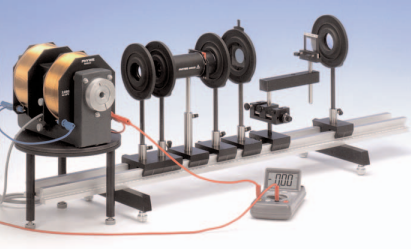
\includegraphics[scale = 0.35]{Figures/setup.png}
        \caption{Experimental set up for determining the elementary charge with the Millikan apparatus}
        \label{fig:setup}
    \end{figure}
    

\section{Theory}
    The main principle of this experiment derives from using the fundamental forces of nature to accomplish our task of find the elementary charge.
    \par
    Charged oil droplets subjected to an electric field and to gravity between the plates of a capacitor are accelerated by application of a voltage. The elementary charge is determined from the velocities in the direction of gravity and in the opposite direction. In the following discussion, we will revisit and highlight the fundamental aspects that will come into play in the experiment.
    \par
    An electric field is the physical field that surrounds electrically-charged particles and exerts force on all other charged particles in the field, either attracting or repelling them. It is a manifestation of the electromagnetic force, one of the most fundamental forces (or interactions) in nature.
    \par
    The viscosity of a fluid is a measure of its resistance to deformation at a given rate. Viscosity can be conceptualized as quantifying the internal frictional force that arises between adjacent layers of fluid that are in relative motion.
    \par 
    In 1851, George Gabriel Stokes derived an expression, now known as Stokes law, for the frictional force – also called drag force – exerted on spherical objects with very small Reynolds numbers in a viscous fluid. The Reynolds number (\textbf{Re}) helps predict flow patterns in different fluid flow situations. At low Reynolds numbers, flows tend to be dominated by laminar (sheet-like) flow, while at high Reynolds numbers flows tend to be turbulent. Stokes' law is derived by solving the Stokes flow limit for small Reynolds numbers of the Navier–Stokes equations.
    \par
    Terminal velocity is the maximum velocity attainable by an object as it falls through a fluid. It occurs when the sum of the drag force ($F_d$) and the buoyancy is equal to the downward force of gravity ($F_G$) acting on the object. Since the net force on the object is zero, the object has zero acceleration, that is, constant velocity.
    \par
    Coming back to the experiment, we observe the rising and falling movement of the charged oil droplets in the electric field of the capacitor. Initially the oil drops are allowed to fall between the plates with the electric field turned off. They very quickly reach a terminal velocity because of friction with the air in the chamber. The field is then turned on and, if it is large enough, some of the drops (the charged ones) will start to rise. (This is because the upwards electric force FE is greater for them than the downwards gravitational force Fg, in the same way bits of paper can be picked by a charged rubber rod). A likely looking drop is selected and kept in the middle of the field of view by alternately switching off the voltage until all the other drops have fallen. The experiment is then continued with this one drop.
    \par
    From Stokes' law, the force $F$ experienced by a sphere of radius $r$ and velocity $v$ in a viscous fluid of viscosity $\eta$ is:
    \begin{equation}
    \label{stokes}
        F = 6 \pi \eta r v
    \end{equation}
    As this spherical droplet of mass $m$, volume $V$ and density $\rho_1$ is also under the influence of earth's gravitational field.
    \begin{equation}
        F =  m \cdot g = \rho_1 \cdot V \cdot g
    \end{equation}
    Now force of buoyancy is given by
    \begin{equation}
        F = \rho_2 \cdot V \cdot g
    \end{equation}
    where $\rho_2$ is the density of air.\\
    The force of electric field is given by
    \begin{equation}
        F = Q \cdot E = Q \cdot \dfrac{U}{d}
    \end{equation}
    where $U$ is the applied voltage across the capacitor with distance between the plates equal to $d$.
    From the sum of the forces affecting a charged particle, the fall and rise velocities of the droplets are obtained.
    \begin{equation}
        v_1 = \dfrac{1}{6 \pi \eta r} \Bigg (Q \cdot E + \dfrac{4}{3} \pi r^3 g (\rho_1 - \rho_2) \Bigg)
    \end{equation}
    \begin{equation}
        v_2 = \dfrac{1}{6 \pi \eta r} \Bigg (Q \cdot E - \dfrac{4}{3} \pi r^3 g (\rho_1 - \rho_2) \Bigg)
    \end{equation}
    Subtraction or addition of these equations gives the radius and the charge of the droplet.\\
    With
    \begin{equation}
        \begin{aligned}
            Q = C_1 \cdot \dfrac{v_1 + v_2}{U}\sqrt{v_1 - v_2} \\
            C_1 = \dfrac{9}{2} \pi d \cdot \sqrt{\dfrac{\eta^3}{g (\rho_1 - \rho_2)}} \\
            C_1 = \SI{2.73e-11}{\kg \cdot \raiseto{1/2} \metre \cdot \raiseto{-1/2} \second}
        \end{aligned}
    \end{equation}
    with
    \begin{equation}
        \begin{aligned}[t]
            r = C_2 \cdot \sqrt{v_1 - v_2} \\
            C_2 = \dfrac{3}{2} \sqrt{\dfrac{\eta}{g (\rho_1 - \rho_2)}} \\
            C_2 = \SI{6.37e-5}{\raiseto{1/2} {(\metre \cdot \second)}}
        \end{aligned}
    \end{equation}
    

\section{Experimental Procedure}
    \begin{enumerate}
        \item Set the capacitor voltage to a value between 300 V and 500 V.
        \item Blow in the oil droplets.
        \item Select an oil droplet and by operating the commutator switch move the droplet between the highest and lowest graduations on the eyepiece micrometer.
        \item Correct the focusing of the microscope if necessary.
        \item Note the following criteria when selecting the droplet:
            \begin{enumerate}
                \item The droplet must not move too fast, then it has a small charge (it should need around one to three seconds for the way of 30 divisions).
                \item The droplet must not move too slowly and should not exhibit any swaying movements. Increase the capacitor voltage if required. 
            \end{enumerate}
        \item Sum together some rise times using the first stopwatch.
        \item Sum together some fall times using the second stopwatch.
        \item The added times should be greater than 5 s in both cases.
    \end{enumerate}
    
    
\section{Observations}
    \begin{enumerate}
        \item Capacitor inter-electrode distance, \\$d = \SI{2.5 \pm 0.01}{\milli \metre}$.
        \item Density of silicone oil, $\rho_1 = \SI{1.03e3}{\kg \raiseto{-3} \metre}$.
        \item Viscosity of air, $\eta = \SI{1.82e-5}{\kg \cdot \raiseto{-1} {(\metre \cdot \second)} }$.
        \item Gravitational acceleration, $g = \SI{9.81}{\metre \per \second \squared}$.
        \item Density of air, $\rho_2 = \SI{1.293}{\kg \cdot \raiseto{-3} \metre}$.
    \end{enumerate}
    \begin{table*}[]
    \caption{\label{tab:data} Measurements on various droplets for determining the elementary charge by the Millikan method. \\$t_1$ and $t_2$ are the fall and rise times of the droplets}
    \begin{ruledtabular}
    \begin{tabular}{cccccccccccccc}
    \hline
    \begin{tabular}[c]{@{}c@{}}$\mathbf{U}$\\ (V)\end{tabular} &
    \begin{tabular}[c]{@{}c@{}}$\mathbf{t_1}$\\ (s)\end{tabular} &
    \begin{tabular}[c]{@{}c@{}}$\mathbf{s_1}$\\ (div.)\end{tabular} &
    \begin{tabular}[c]{@{}c@{}}$\mathbf{t_2}$\\ (s)\end{tabular} &
    \begin{tabular}[c]{@{}c@{}}$\mathbf{s_2}$\\ (div.)\end{tabular} &
    \begin{tabular}[c]{@{}c@{}}$\mathbf{s_1}$\\ (mm)\end{tabular} &
    \begin{tabular}[c]{@{}c@{}}$\mathbf{s_2}$\\ (mm)\end{tabular} &
    \begin{tabular}[c]{@{}c@{}}$\mathbf{v_1}$\\ (m/s)\end{tabular} &
    \begin{tabular}[c]{@{}c@{}}$\mathbf{v_2}$\\ (m/s)\end{tabular} &
    \begin{tabular}[c]{@{}c@{}}$\mathbf{v_1 - v_2}$\\ (m/s)\end{tabular} &
    \begin{tabular}[c]{@{}c@{}}$\mathbf{r}$\\ (m)\end{tabular} &
    \begin{tabular}[c]{@{}c@{}}$\mathbf{Q}$\\ (As)\end{tabular} &
    n &
    \begin{tabular}[c]{@{}c@{}}$\mathbf{e}$\\ (As)\end{tabular} \\ \hline
    \hline
    360 & 5.72 & 60  & 8.42 & 60 & 1.96 & 1.78 & 3.43E-04 & 2.11E-04 & 1.31E-04 & 7.30E-07 & 4.81E-19 & 3 & 1.60E-19 \\
    360 & 6.61 & 60  & 8.39 & 60 & 1.96 & 1.78 & 2.97E-04 & 2.12E-04 & 8.44E-05 & 5.85E-07 & 3.54E-19 & 2 & 1.77E-19 \\
    360 & 6.29 & 60  & 9.17 & 60 & 1.96 & 1.78 & 3.12E-04 & 1.94E-04 & 1.17E-04 & 6.90E-07 & 4.16E-19 & 3 & 1.39E-19 \\
    360 & 5.78 & 60  & 8.43 & 60 & 1.96 & 1.78 & 3.39E-04 & 2.11E-04 & 1.28E-04 & 7.21E-07 & 4.72E-19 & 3 & 1.57E-19 \\
    360 & 6.03 & 60  & 8.84 & 60 & 1.96 & 1.78 & 3.25E-04 & 2.01E-04 & 1.24E-04 & 7.08E-07 & 4.44E-19 & 3 & 1.48E-19 \\
    360 & 6.83 & 90  & 8.56 & 60 & 2.94 & 1.78 & 4.30E-04 & 2.08E-04 & 2.23E-04 & 9.50E-07 & 7.22E-19 & 5 & 1.44E-19 \\
    360 & 5.93 & 60  & 9.56 & 60 & 1.96 & 1.78 & 3.31E-04 & 1.86E-04 & 1.44E-04 & 7.65E-07 & 4.71E-19 & 3 & 1.57E-19 \\
    360 & 6.50 & 60  & 8.93 & 60 & 1.96 & 1.78 & 3.02E-04 & 1.99E-04 & 1.02E-04 & 6.44E-07 & 3.84E-19 & 2 & 1.92E-19 \\
    360 & 6.43 & 60  & 8.52 & 60 & 1.96 & 1.78 & 3.05E-04 & 2.09E-04 & 9.59E-05 & 6.24E-07 & 3.82E-19 & 2 & 1.91E-19 \\
    360 & 5.88 & 60  & 8.78 & 60 & 1.96 & 1.78 & 3.33E-04 & 2.03E-04 & 1.31E-04 & 7.28E-07 & 4.65E-19 & 3 & 1.55E-19 \\
    460 & 7.33 & 90  & 6.45 & 60 & 2.94 & 1.78 & 4.01E-04 & 2.76E-04 & 1.25E-04 & 7.13E-07 & 4.49E-19 & 3 & 1.50E-19 \\
    460 & 8.23 & 120 & 8.45 & 60 & 3.92 & 1.78 & 4.76E-04 & 2.11E-04 & 2.66E-04 & 1.04E-06 & 6.64E-19 & 4 & 1.66E-19 \\
    460 & 7.83 & 90  & 7.68 & 60 & 2.94 & 1.78 & 3.75E-04 & 2.32E-04 & 1.44E-04 & 7.64E-07 & 4.32E-19 & 3 & 1.44E-19 \\
    460 & 7.91 & 120 & 9.34 & 60 & 3.92 & 1.78 & 4.96E-04 & 1.91E-04 & 3.05E-04 & 1.11E-06 & 7.11E-19 & 4 & 1.78E-19 \\
    460 & 7.27 & 120 & 8.84 & 60 & 3.92 & 1.78 & 5.39E-04 & 2.01E-04 & 3.38E-04 & 1.17E-06 & 8.08E-19 & 5 & 1.62E-19 \\
    460 & 8.15 & 120 & 8.59 & 60 & 3.92 & 1.78 & 4.81E-04 & 2.07E-04 & 2.74E-04 & 1.05E-06 & 6.76E-19 & 4 & 1.69E-19 \\
    460 & 8.06 & 90  & 9.14 & 90 & 2.94 & 2.67 & 3.65E-04 & 2.92E-04 & 7.26E-05 & 5.43E-07 & 3.32E-19 & 2 & 1.66E-19 \\
    460 & 7.78 & 90  & 9.66 & 90 & 2.94 & 2.67 & 3.78E-04 & 2.76E-04 & 1.01E-04 & 6.42E-07 & 3.91E-19 & 2 & 1.96E-19 \\
    460 & 8.25 & 120 & 9.13 & 90 & 3.92 & 2.67 & 4.75E-04 & 2.92E-04 & 1.83E-04 & 8.61E-07 & 6.16E-19 & 4 & 1.54E-19 \\
    460 & 7.45 & 90  & 7.55 & 60 & 2.94 & 1.78 & 3.95E-04 & 2.36E-04 & 1.59E-04 & 8.03E-07 & 4.72E-19 & 3 & 1.57E-19 \\
    560 & 6.32 & 90  & 7.36 & 60 & 2.94 & 1.78 & 4.65E-04 & 2.42E-04 & 2.23E-04 & 9.52E-07 & 5.15E-19 & 3 & 1.72E-19 \\
    560 & 7.34 & 120 & 9.78 & 90 & 3.92 & 2.67 & 5.34E-04 & 2.73E-04 & 2.61E-04 & 1.03E-06 & 6.36E-19 & 4 & 1.59E-19 \\
    560 & 7.65 & 120 & 9.01 & 90 & 3.92 & 2.67 & 5.12E-04 & 2.96E-04 & 2.16E-04 & 9.36E-07 & 5.80E-19 & 4 & 1.45E-19 \\
    560 & 7.12 & 90  & 8.45 & 90 & 2.94 & 2.67 & 4.13E-04 & 3.16E-04 & 9.69E-05 & 6.27E-07 & 3.50E-19 & 2 & 1.75E-19 \\
    560 & 7.86 & 120 & 8.70 & 90 & 3.92 & 2.67 & 4.99E-04 & 3.07E-04 & 1.92E-04 & 8.82E-07 & 5.44E-19 & 3 & 1.81E-19 \\
    560 & 7.91 & 120 & 8.90 & 90 & 3.92 & 2.67 & 4.96E-04 & 3.00E-04 & 1.96E-04 & 8.91E-07 & 5.42E-19 & 3 & 1.81E-19 \\
    560 & 8.09 & 90  & 7.99 & 90 & 2.94 & 2.67 & 3.63E-04 & 3.34E-04 & 2.92E-05 & 3.44E-07 & 1.84E-19 & 1 & 1.84E-19 \\
    560 & 7.67 & 120 & 8.32 & 90 & 3.92 & 2.67 & 5.11E-04 & 3.21E-04 & 1.90E-04 & 8.78E-07 & 5.59E-19 & 3 & 1.86E-19 \\
    560 & 7.17 & 90  & 9.01 & 90 & 2.94 & 2.67 & 4.10E-04 & 2.96E-04 & 1.14E-04 & 6.79E-07 & 3.67E-19 & 2 & 1.84E-19 \\
    560 & 8.34 & 120 & 9.34 & 90 & 3.92 & 2.67 & 4.70E-04 & 2.86E-04 & 1.84E-04 & 8.64E-07 & 5.00E-19 & 3 & 1.67E-19 \\ \hline
    \end{tabular}
    \end{ruledtabular}
    \end{table*}
    

\section{Results and discussions}
    The following is the plot of radius of droplets vs the charge of droplets.  It  is  clearly  evident  from  the  plot  that distinct steps are seen in Q, which implies the droplets acquire only integral multiples of the elementary charge $e$.  On approximately estimating the levels, i.e.  multiples (n),  we  come  to  see that  the  data  almost  matches  our assumed model.
    \begin{figure}[h!]
        \centering
        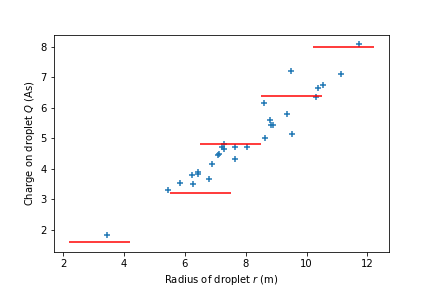
\includegraphics[scale = 0.55]{Figures/plot.png}
        \caption{Measurements on various droplets for determining the elementary charge by the Millikan method.}
        \label{fig:plot}
    \end{figure}
    From table (\ref{tab:data}) the average value of $e$ obtained is \boxed{$\SI{1.66e-19}{\coulomb}$}.


\section{Error Analysis}
We would be calculating the standard deviation of the values of $e$ obtained.
The formula for standard deviation is
\begin{equation}
    \sigma = \sqrt{\dfrac{\Sigma (x_i - \mu)^2}{N - 1}}
\end{equation}
We have average, $\mu = \SI{1.66e-19}{\coulomb}$ and number of values, $N = 30$. Putting in the values we get, 
$\sigma = \SI{0.16e-19}{\coulomb}$.
\section{Conclusions}
\begin{enumerate}
    \item The  net  charge  on  an  oil  droplet  is  an  integral multiple of the elementary charge or charge of an electron (e).
    \item The value of this elementary charge is found to be (after rounding off to most significant digit) $\mathbf{1.7\pm 0.2\times 10^{-19}  C}$.
    \item Although the literature value of e is $1.602 \times 10^{-19} C$, the observed value is quite close to this and falls within 1 $\%$ of the literature value.
    \item The error seen in the data can be accredited to the experimental error, since no systematic error was observed in the instruments used. Some of the error may also be accredited to human error, which occurs when we record the falling and rising times of the droplets using stopwatch.
\end{enumerate}





% Produces the bibliography via BibTeX.

\end{document}
%
% ****** End of file apssamp.tex ******
